%% Chapter 1
\chapter{Introduction} % Main chapter title
\label{chapterIntroduction} 
%%%%%%%%%%%%%%%%%%%%%%%%%%%%%%%%%%%%%%%%%%%%%%%%%%
%%%%%%%%%%%                                                     %%%%%%%%%%%%%%%%%%%%%%%%%%%
%%%%%%%%%%%           1.1   Consumer \gls{RGBD} Cameras                   %%%%%%%%%%%%%%%%%%%%
%%%%%%%%%%%                                                     %%%%%%%%%%%%%%%%%%%%%%%%
%%%%%%%%%%%%%%%%%%%%%%%%%%%%%%%%%%%%%%%%%%%%%%%%%%%
\section{RGBD Cameras}
\indent
A Red-Green-Blue-Depth (\gls{RGBD}) camera is a sensing system that captures RGB images along with per-pixel depth information. Usually it is simply a combination of a RGB sensor and a depth sensor with an alignment algorithm. For instance, the PrimeSense's technology had been originally applied to gaming, with user interfaces based on gesture recognition instead of using a controller (also called Natural User Interface, \gls{NUI} \cite{BraveNUIworld_2011}). PrimeSense was best known for licensing the hardware design and chip used in Microsoft's first generation of Kinect motion-sensing system for the Xbox 360 in 2010 \cite{PrimeSenseInfo_2013}. The PrimeSense sensor projects an infrared speckle pattern, which will then be captured by an infrared camera in the sensor. A special microchip is employed to compare the captured speckle pattern part-by-part to reference patterns stored in the device, which were captured previously at known depths. The final per-pixel depth will be estimated based on which reference patterns the captured pattern matches best \cite{Krystof12}. Other than the first generation of Kinect camera, Asus Xtion PRO sensor, another consumer \gls{NUI} application product, has also applied the PrimeSense's technology \cite{AsusXtion_2013}.
\\\indent%
As a competitor \cite{evaluationBetween_2015} of PrimeSense Structured Light technology, time-of-flight technology had been applied into PMD[Vision] CamCube cameras and 3DV's ZCam cameras. Based on known speed of light, Time-of-Flight (\gls{ToF}) camera resolves distance by measuring the \enquote{time cost} of a special light signal traveling between the camera and target for every single point. The \enquote{time cost} variable that \gls{ToF} camera measures is the phase shift between the illumination and reflection, which will be translated to distance \cite{TimeOfFlight}. To detect the phase shifts, a light source is pulsed or modulated by a continuous wave, typically a sinusoid or square wave. The \gls{ToF} camera illumination is typically from a LED or a solid-state laser operating in the near-infrared range invisible to human eyes. Fabrizio \textit{et al}. \cite{depthTechCompare_2011} compared the time-of-flight (PMD[Vision] CamCube) camera and PrimeSense (first generation Kinect) camera in 2011. He showed that the time-of-flight technology is more accurate and claimed that the time-of-flight technology will not only be extended to support colours and higher frame sizes, but also rapidly drop in price. %
% In 2009, 3DV agreed to sell its ZCam assets to Microsoft.
In 2010, it was announced that Microsoft would acquire Canesta for an undisclosed amount \cite{Canesta_2010}. %
And in 2013,  Microsoft released the Xbox One, whose \gls{NUI} sensor \gls{KinectV2} features a wide-angle Canesta \gls{ToF} camera.
\\\indent
Unlike the PrimeSense's speckle pattern or \gls{KinectV2}'s \gls{ToF}, Intel RealSense camera utilizes stereo vision \cite{RealSense01_2015}. Its sensor actually has three cameras: two infrared (\gls{IR}) cameras (left and right), and one RGB camera. Additionally, RealSense camera also has an \gls{IR} laser projector to help the stereo vision recognize depth at unstructured surfaces. Compared with \gls{KinectV2} camera, RealSense camera is more like a desktop usage to capture faces or even finger gestures, whereas the \gls{KinectV2} could do better to capture the full body actions with all joints \cite{RealSense02_2016}. The effective distances of \gls{KinectV2} and RealSense hardwares are different. The \gls{KinectV2} is optimized to 0.5m \texttildelow 4.5m, while RealSense are designed for 0.2m \texttildelow 1.2m depends on different devices.

%%%%%%%%%%%%%%%%%%%%%%%%%%%%%%%%%%%%%%%%%%%%%%%%%%
%%%%%%%%%%%                                                                %%%%%%%%%%%%%%%%%
%%%%%%%%%%     1.2  Human Computer Interface                %%%%%%%%%%%%%%%%%%%%
%%%%%%%%%%%                                                                %%%%%%%%%%%%%%%%%%
%%%%%%%%%%%%%%%%%%%%%%%%%%%%%%%%%%%%%%%%%%%%%%%%%%%
\section{Human Computer Interface}
%%
%%
%%
%% gesture recognition
\indent
Gesture recognition is one of the hottest sustained research activities in the area of \gls{HCI} \cite{NIRGesture14}. It has a wide area of application including human machine interaction, sign language, immersive game technology \textit{etc}. Being a significant part in non-verbal communication, hand gestures are playing vital role in our daily life. Hand Gesture recognition system provides us an innovative, natural, user friendly way of interaction with the computer. By keeping in mind the similarities of human hand shape with four fingers and one thumb, Meenakshi \cite{gestureRecognition12} presents a real time system for hand gesture recognition on the basis of detection of some meaningful shape based features like orientation, center of mass (centroid), status of fingers, thumb in terms of raised or folded fingers of hand and their respective location in image. Since gestures based on hand and finger movements can be robustly understood by computers by using a special \gls{3D} \gls{IR} camera, users are allowed to play games and interact with computer applications in natural and immersive ways that improve the user experience. 
\\\indent
Kam \textit{et al}. \cite{KinectGesture12} developed a real-time gesture-driven human computer interface using the \gls{KinectV1} camera and achieved close to 100\% practical recognition rates. After Kam, a Kinect-based calling gesture recognition scenario is proposed by Xinshuang  \textit{et al}. \cite{gestureKinect14} for taking order service of an elderly care robot. Its proposed scenarios are designed mainly for helping non expert users like elderly to call service robot for their service request. In order to facilitate elderly service, natural calling gestures are designed to interact with the robot. Figure~\ref{KinectBasedCallingGesture} shows the evaluation of gesture recognition when sitting on chair. Individual subjects are segmented out from \gls{3D} point clouds acquired by Microsoft Kinect, skeletons are generated for each subject. And face detection is applied to identify whether the segment is human or not, and specific natural calling gestures are designed based on skeleton joints. %
\\\indent
\begin{figure}[t]
\centering
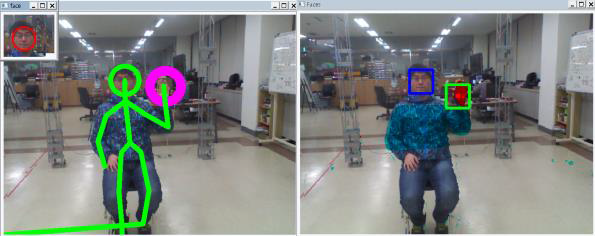
\includegraphics[width=\textwidth]{KinectBasedCallingGesture}
\caption{Calling Gesture Recognition Using Kinect \cite{gestureKinect14}}
\label{KinectBasedCallingGesture}
\end{figure}%
%
\begin{figure}[t]
\centering
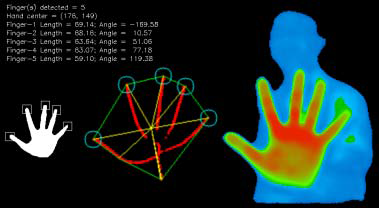
\includegraphics[width=\textwidth]{FingerDetectionUsingDepthData}
\caption{Finger Detection using Depth Data \cite{NIRGesture14}}
\label{FingerDetectionUsingDepthData}
\end{figure}%
Dan \textit{et al}. \cite{NIRGesture14} proposed another smart and real-time depth camera based on a new depth generation principle. A monotonic increasing and decreasing function is used to control the frequency and duty-cycle of the \gls{NIR} illumination pulses. The adjusted light pulses reflect off of the object of interest and are captured as a series of images. A reconfigurable hardware architecture calculates the depth-map of the visible face of the object in real-time from a number of images. The final depth map is then used for gesture detection, tracking and recognition. Figure~\ref{FingerDetectionUsingDepthData} shows an example extraction of hand skeleton. In 2013, Jaehong \textit{et al}. \cite{InteractiveManipulation_2013} develop and implement a Kinect-based \gls{3D} gesture recognition system for interactive
manipulation of \gls{3D} objects in educational visualization softwares. 
\\\indent%
%
%%%%
%%%
%%%
%%% \gls{SLAM} --> accuracy
%%%
%%% indoor perception, \gls{SLAM}, 
\section{Robust Vision}
\indent
\gls{RGBD} cameras own great credits in mobile robotics, building dense \gls{3D} maps of indoor environments. Such maps have applications in robot navigation, manipulation, semantic mapping, and telepresence. Peter \textit{et al}. \cite{indorMappingRGBD_2014} present a detailed \gls{RGBD} mapping system that utilizes a joint optimization algorithm combining visual features and shape-based alignment. Building on best practices in Simultaneous Localization And Mapping (\gls{SLAM}) and computer graphics makes it possible to build and visualize accurate and extremely rich \gls{3D} maps with \gls{RGBD} cameras. Visual and depth information are also combined for view-based loop closure detection, followed by pose optimization to achieve globally consistent maps. \gls{SLAM} is the process of generating a model of the environment around a robot or sensor, while simultaneously estimating the location of the robot or sensor relative to the environment. \gls{SLAM} has been performed in many ways, which can be categorized generally by their focus on localization or environment mapping \cite{SLAMintro_2015}. \gls{SLAM} systems focused on localizing the sensor accurately, relative to the immediate environment, make use of sparse sensor data to locate the sensor. Using range sensors such as scanning laser range-finders \cite{laserSLAM_2011}, LiDAR and SONAR \cite{sonarSLAM_2013}, many robot applications use \gls{SLAM} systems only to compute the distance from the sensor to the environment. \gls{SLAM} systems focused on mapping use dense sensor output to create a high-fidelity \gls{3D} map of the environment, while using those data to also compute relative location of the sensor \cite{KinectFusion_2011, mapSLAM_2013}. Many modern \gls{SLAM} algorithms combine both approaches, usually by extracting sparse features from the sensor and using these for efficiently computing the location of the sensor. This position is then used to construct a map from dense sensor data. 
\\\indent
With a consumer \gls{RGBD} camera providing both color images and dense depth maps at full video frame rate, there appears a novel approach to \gls{SLAM} that combines the scale information of \gls{3D} depth sensing with the strengths of visual features to create dense \gls{3D} environment representations, which is called \gls{RGBD} \gls{SLAM}. Felix \textit{et al}. \cite{RGBDSLAM01_2012} gives an open source approach to visual \gls{SLAM} from \gls{RGBD} sensors, which extracts visual keypoints from the color images and uses the depth images to localize them in \gls{3D}. %
%
\begin{figure}[t]
\centering
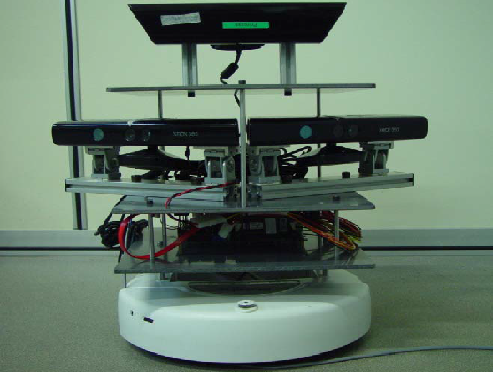
\includegraphics[width=0.5\textwidth]{threeKinect}
\caption{\gls{SLAM} system with Only \gls{RGBD} Cameras \cite{RGBDSLAMsystem_2013}}
\label{threeKinect}
\end{figure}%
%
Maohai \textit{et al}. \cite{RGBDSLAMsystem_2013} builds an efficient \gls{SLAM} system using three \gls{RGBD} sensors. As shown in Fig.~\ref{threeKinect}, one Kinect looking up toward the ceiling can track the robot's trajectory through visual odometry method, which provide more accurate motion estimation compared to wheel motion measurement without being disturbed under wheel slippage. And the other two contiguous horizontal Kinects can provide wide range scans, which ensure more robust scan matching in the RBPF-\gls{SLAM} framework. %
\\\indent
%
Also using \gls{RGBD} sensor for \gls{SLAM}, Kathia \textit{et al}. \cite{bundleSLAMRGBD_2015} presents a constraint bundle adjustment which allows to easily combine depth and visual data in cost function entirely expressed in pixel. In order to enhance the instantaneity of \gls{SLAM} for indoor mobile robot, Guanxi \textit{et al}. \cite{indorRGBDSLAM_2015} proposed a \gls{RGBD} \gls{SLAM} method based on Kinect camera, which combined Oriented FAST and Rotated BRIEF (ORB) algorithm with Progressive Sample Consensus (PROSAC) algorithm to execute feature extracting and matching. %
%
%
ORB algorithm which has better property than many other feature descriptors was used for extracting feature. At the same time, ICP algorithm was adopted for coarse registration of the point clouds, and PROSAC algorithm which is superior than RANSAC in outlier removal was employed to eliminate incorrect matching. To make the result more accurate, pose-graph optimization was achieved based on General Graph Optimization (g2o) framework. Figure~\ref{3DpointCloudMapOfLab} shows the \gls{3D} volumetric map of the lab, which can be directly used to navigate robots.
\\\indent%
%%
%A robot, for example, needs to know its location in the world to navigate between places. This problem is a classical and challenging chicken-and-egg problem because localizing the camera in the world requires the \gls{3D} model of the world, and building the \gls{3D} model in turn requires the pose of the camera. Therefore, both the camera trajectory and the \gls{3D} model need to be estimated at the same time.
\begin{figure}[t]
\centering
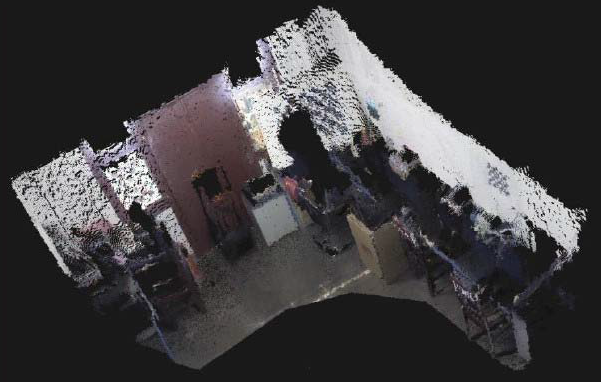
\includegraphics[width=0.7\textwidth]{3DpointCloudMapOfLab}
\caption{\gls{3D} Map of \gls{RGBD}-\gls{SLAM} with ORB and PROSAC \cite{indorRGBDSLAM_2015}}
\label{3DpointCloudMapOfLab}
\end{figure}%
%
\gls{RGBD} camera is also famous in application of doing visual odometry on autonomous flight of a micro air vehicle (MAV), helping acquire \gls{3D} models of the environment and estimate the camera pose with respect to the environment model. Visual odometry generally has unbounded global drift while estimating local motion. To bound estimation error, it can be integrated with \gls{SLAM} algorithms, which employ loop closing techniques to detect when a vehicle revisits a previous location. A computationally inexpensive \gls{RGBD}-\gls{SLAM} solution tailored to the application on autonomous MAVs is discussed by Sebastian and Andreas \cite{RGBDSLAMmav_2013}, which enables our MAV to fly in an unknown environment and create a map of its surroundings completely autonomously, with all computations running on its onboard computer. Figure~\ref{RGBD_SLAM_MAV} shows the MAC with an \gls{RGBD} sensor (the first generation of Kinect) mounted. And Fig.~\ref{mavReconstruction} shows the reconstruction based on the full point clouds, with the estimated trajectory shown in red dots. 
%
\\\indent
%
\begin{figure}[t]
\centering
\subfloat[RGBD UAV]{
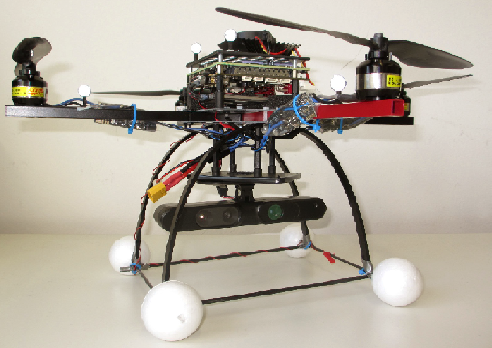
\includegraphics[height=0.4\textwidth , width = 0.5\textwidth]{RGBD_SLAM_MAV}
\label{RGBD_SLAM_MAV}}
\subfloat[Reconstruction and Estimated Trajectory]{
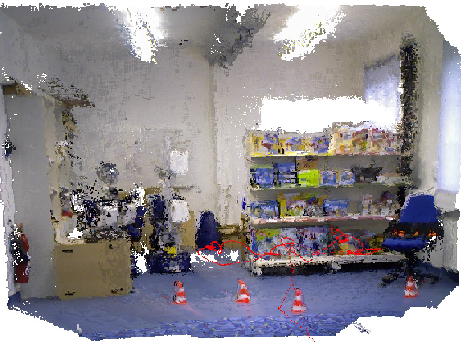
\includegraphics[height=0.4\textwidth , width = 0.5\textwidth]{mavReconstruction}
\label{mavReconstruction}}
%\qquad
\caption{RGBD-SLAM for Autonomous MAVs \cite{RGBDSLAMmav_2013}}
\label{autoRGBD_SLAM_MAV}
\end{figure}%
% Volumetric Reconstruction and Virtual Reality : \gls{3D} printing, Kinect fusion
% KinectFusion, \gls{3D} printing
\section{3D Scanning and Printing}
\gls{RGBD} sensors can be used on a much smaller scale than \gls{SLAM} to create more detailed, volumetric reconstructions of objects and smaller environments, which opens a new world to the fast \gls{3D} printing. \gls{3D} printing is an additive technology in which \gls{3D} objects are created using layering techniques of different materials, such as plastic, metal, \textit{etc}.  It has been around for decades, but only recently is available and famous among the general public. The first \gls{3D} printing technology developed in the 1980's was stereolithography (SLA) \cite{Patent3Dprinting86}. This technique uses an ultraviolet (UV) curable polymer resin and an UV laser to build each layer one by one. Since then other \gls{3D} printing technologies have been introduced. Nowadays, some companies like iMaterialise or Shapeways offer \gls{3D} printing services where you can simply upload your CAD model on-line, choose a material and in a few weeks your \gls{3D} printed object will be delivered to your address. This procedure is quite straight-forward when you got your CAD model. However, \gls{3D} shape design tends to be a long and tedious process, with the design of a detailed \gls{3D} part usually requiring multiple revisions. Fabricating physical prototypes using low cost \gls{3D} fabrication technologies at intermediate stages of the design process is now a common practice, which helps the designer discover errors, and to incrementally refine the design \cite{3DModelingForPrinting15}. Most often, implementing the required changes directly in the computer model, within the \gls{3D} modeling software, is more difficult and time consuming than modifying the physical model directly using hand cutting, caving and sculpting tools, power tools, or machine tools. When one of the two models is modified, the changes need to be transferred to the other model, a process we refer to as synchronization. 
\\\indent
KinectFusion \cite{KinectFusionIzadi_2011}, a framework that allows a user to create a detailed \gls{3D} reconstruction of an object or a small environment in real-time using Microsoft Kinect sensor, has garnered a lot of attention in the reconstruction and modeling field. It enables a user holding and moving a standard Kinect camera to rapidly create detailed \gls{3D} reconstructions of an indoor scene. Not only an entire scene, a specific smaller physical object could also be cleanly segmented from the background model simply by moving the object directly. Figure~\ref{FastDirectObjectSegmentation} shows how the interested object (a teapot) is accurately segmented from the background by physically removed. The sub-figure (A) shows surface normals, and sub-figure (B) is the texture mapped model. %
%
\begin{figure}[t]
\centering
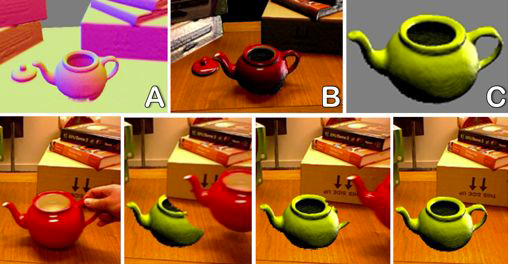
\includegraphics[width=\textwidth]{FastDirectObjectSegmentation}
\caption{Object Segmentation in KinectFusion \cite{KinectFusionIzadi_2011}}
\label{FastDirectObjectSegmentation}
\end{figure}%
%
Nadia \textit{et al}. \cite{3DPrintingFrom3DSensing13} proposed and introduced a from-Sense-to-Print system that can automatically generate ready-to-print \gls{3D} CAD models of objects or humans from \gls{3D} reconstructions using the low-cost Kinect sensor. Further, Ammar and Gabriel \cite{3DModelingForPrinting15} addresses the problem of synchronizing the computer model to changes made in the physical model by \gls{3D} scanning the modified physical model, automatically detecting the changes, and updating the computer model. A new method is proposed that allows the designer to move fluidly from the physical model (for example his \gls{3D} printed object, or his carved object) to the computer model. In the proposed process the physical modification applied by the designer to the physical model are detected by \gls{3D} scanning the physical model and comparing the scan to the computer model. Then the changes are reflected in the computer model. The designer can apply further changes either to the computer model or to the physical model. Changes made to the computer model can be synchronized to the physical model by \gls{3D} printing a new physical model.
%
%
%%%%%%%%%%%%%%%%%%%%%%%%%%%%%%%%%%%%%%%%%%%%%%%%%%
%%%%%%%%%%                                                     %%%%%%%%%%%%%%%%%%%%%%%%%%%
%%%%%%%%%%  1.3   Calibration of \gls{RGBD} Cameras         %%%%%%%%%%%%%%%%%%%%%%%%
%%%%%%%%%%                                                     %%%%%%%%%%%%%%%%%%%%%%%%
%%%%%%%%%%%%%%%%%%%%%%%%%%%%%%%%%%%%%%%%%%%%%%%%%%%%%%%
\section{RGBD Cameras' Calibration and 3D Reconstruction on GPU}
\label{sectionRGBDcameraCalibration}
\indent
 \begin{figure}[b]
%\centering
\subfloat[Front View]{
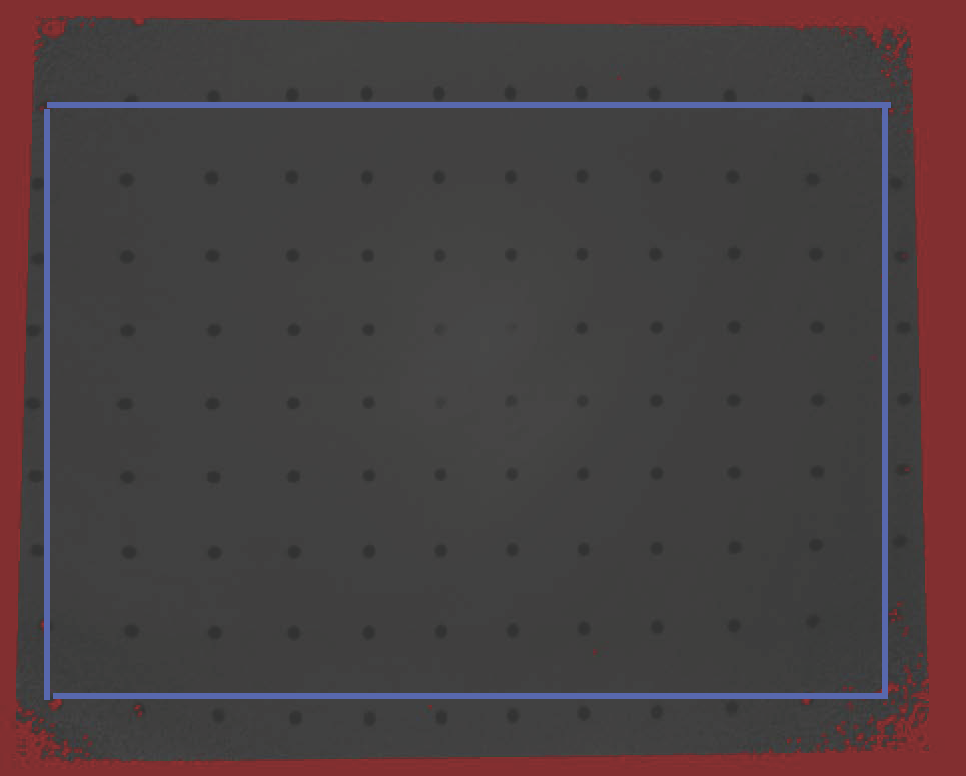
\includegraphics[height=0.42\textwidth]{NIR_by_Depth_front}
\label{NIR_by_Depth_front}}
\subfloat[Side View]{
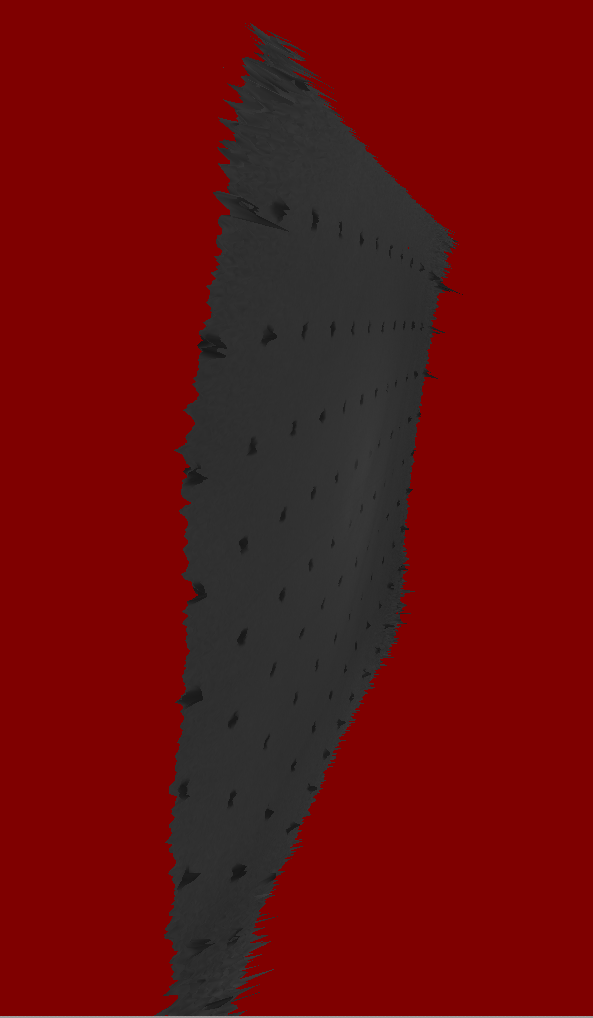
\includegraphics[height=0.42\textwidth , width = 0.4\textwidth]{NIR_by_Depth_LeftSide}
\label{NIR_by_Depth_LeftSide}}
%\qquad
\caption{\gls{KinectV2} \gls{NearIR} \gls{3D} Reconstruction in Camera Space}
\label{NearIR}
\end{figure}%
%
As discussed above, applications like \gls{RGBD}-\gls{SLAM} and KinectFusion apply \gls{3D} reconstruction techniques using an \gls{RGBD} camera, in which an RGB sensor offers color values and a depth sensor measures objects' distances (\(\gls{D}\) or \(\gls{cameraZ}\)). \gls{RGBD} cameras, \text{e.g.} \gls{KinectV2}, offer the horizontal and vertical field of view (\gls{FoV})s of the sensors based on a pinhole camera model, from which a proportional per-pixel beam equation (from \(\gls{cameraZ}\) to \(\gls{cameraX}/\gls{cameraY}\)) could be derived. It is not hard to do \gls{3D} reconstruction in camera space naturally on \gls{GPU} with the help of the proportional per-pixel beam equations; however, the \gls{3D} reconstructed image in that case will be deformed a lot by distortions. Figure~\ref{NearIR} shows the \gls{KinectV2} \gls{NearIR} \gls{3D} reconstruction in camera space, when observing a canvas hung on a flat wall printed with uniform grid ground-dots pattern. In the front view, a blue rectangle is drawn based on four corner dot-clusters, which reflects lens distortions (the uniformed distribution of the captured dot-clusters). While in the side view, a blue straight line added on the side of \gls{3D} reconstruction, which shows the unflatness of captured \enquote{flat wall}. The deformation in the side view is probably caused by the various resolutions of depth sensor on per-pixel basis, which we will call as \emph{depth distortion} in this thesis. In order to get undistorted \gls{3D} images, camera calibration is necessary before a camera being employed.%
\\\indent%
%For decades, much work on camera calibration has been done, starting from the photogrammetry community \cite{photogrammetry01_1971, photogrammetry02_1975}, to computer vision (\cite{Tsai1987, treeDcalibration1_1993, Zhengyou04} to cite a few). After the release of the low-cost Microsoft Kinect, a lot of researchers focus their calibrations specially on \gls{RGBD} cameras (\textit{e.g.}, Kinect). Jan \textit{et al}. \cite{KinectCali01_2011} analyze Kinect as a \gls{3D} measuring device, experimentally investigate depth measurement resolution and error properties and make a quantitative comparison of Kinect accuracy with stereo reconstruction from SLR cameras and a \gls{3D}-TOF camera. Using small data sets of Kinect, Carolina \textit{et al}. \cite{KinectCali02_2013} present a new method for calibrating a color-depth camera pair, which prevents the calibration from suffering a drift in scale. Aaron \textit{et al}. \cite{KinectCali03_2015} presented a novel multi-Kinect calibration algorithm that only requires a user to move single spherical object in front of the Kinects observed from multiple viewpoints.
Camera calibrations usually use calibration objects, which could be assigned world space coordinates (\(\gls{worldX}/\gls{worldY}/\gls{worldZ}\)) to help remove distortions. For decades, much work on camera calibration has been done, starting from the photogrammetry community \cite{photogrammetry01_1971, photogrammetry02_1975}, to computer vision \cite{Tsai1987, treeDcalibration1_1993, Zhengyou04}. And the combination of a pinhole-camera matrix with a distortion removal vector (which contains five high-order polynomial parameters) are widely known as important tools in camera calibration; however, there need to be a lot calculations in the \gls{GPU} fragment shader based on those parameters from both pinhole-camera matrix and distortion removal vector. And we would like to find a simple method with fewer calculations when generating the \gls{3D} coordinates. Similar with the per-pixel \emph{proportional} beam equations in camera space reconstruction on \gls{GPU}, Kai \cite{Kai10} derived more common \emph{linear} beam equations (from \(\gls{worldX}\) to \(\gls{worldY}/\gls{worldZ}\)) directly from the pinhole-camera matrix, on the basis of per-pixel. That \emph{linear} beam equations make it possible to show world space \gls{3D} reconstruction naturally on \gls{GPU}, but it did not contains infos about lens distortion correction. 
\\\indent
%
Our goal is to draw undistorted \gls{3D} reconstruction on \gls{GPU} with the fewest calculations. Inspired by Kai, we will build up a rail calibration system to support the per-pixel \(\gls{D}\) to \(\gls{worldZ}\) mapping, such that Kai's per-pixel \(\gls{worldX}\) to \(\gls{worldY}/\gls{worldZ}\) linear mappings could be applied during the \gls{3D} reconstruction on \gls{GPU}. We will call this new method \textit{per-pixel calibration}. As shown in Fig.~\ref{trackingModuleOnKinectV2CalibrationSystem}, the camera observing the uniform grid dots pattern is mounted on a rail, which is perpendicular to pattern on the wall. A laser distance measurer will be used to supply accurate per-frame \(\gls{worldZ}\), so that the per-pixel \(\gls{D}\) to \(\gls{worldZ}\) mapping could handle \emph{depth distortion}. As long as the undistorted dense \(\gls{worldX}/\gls{worldY}\) could be acquired, we will be able determine the parameters of per-pixel \emph{linear} beam equations.
\\\indent
\begin{figure}[t]
\centering
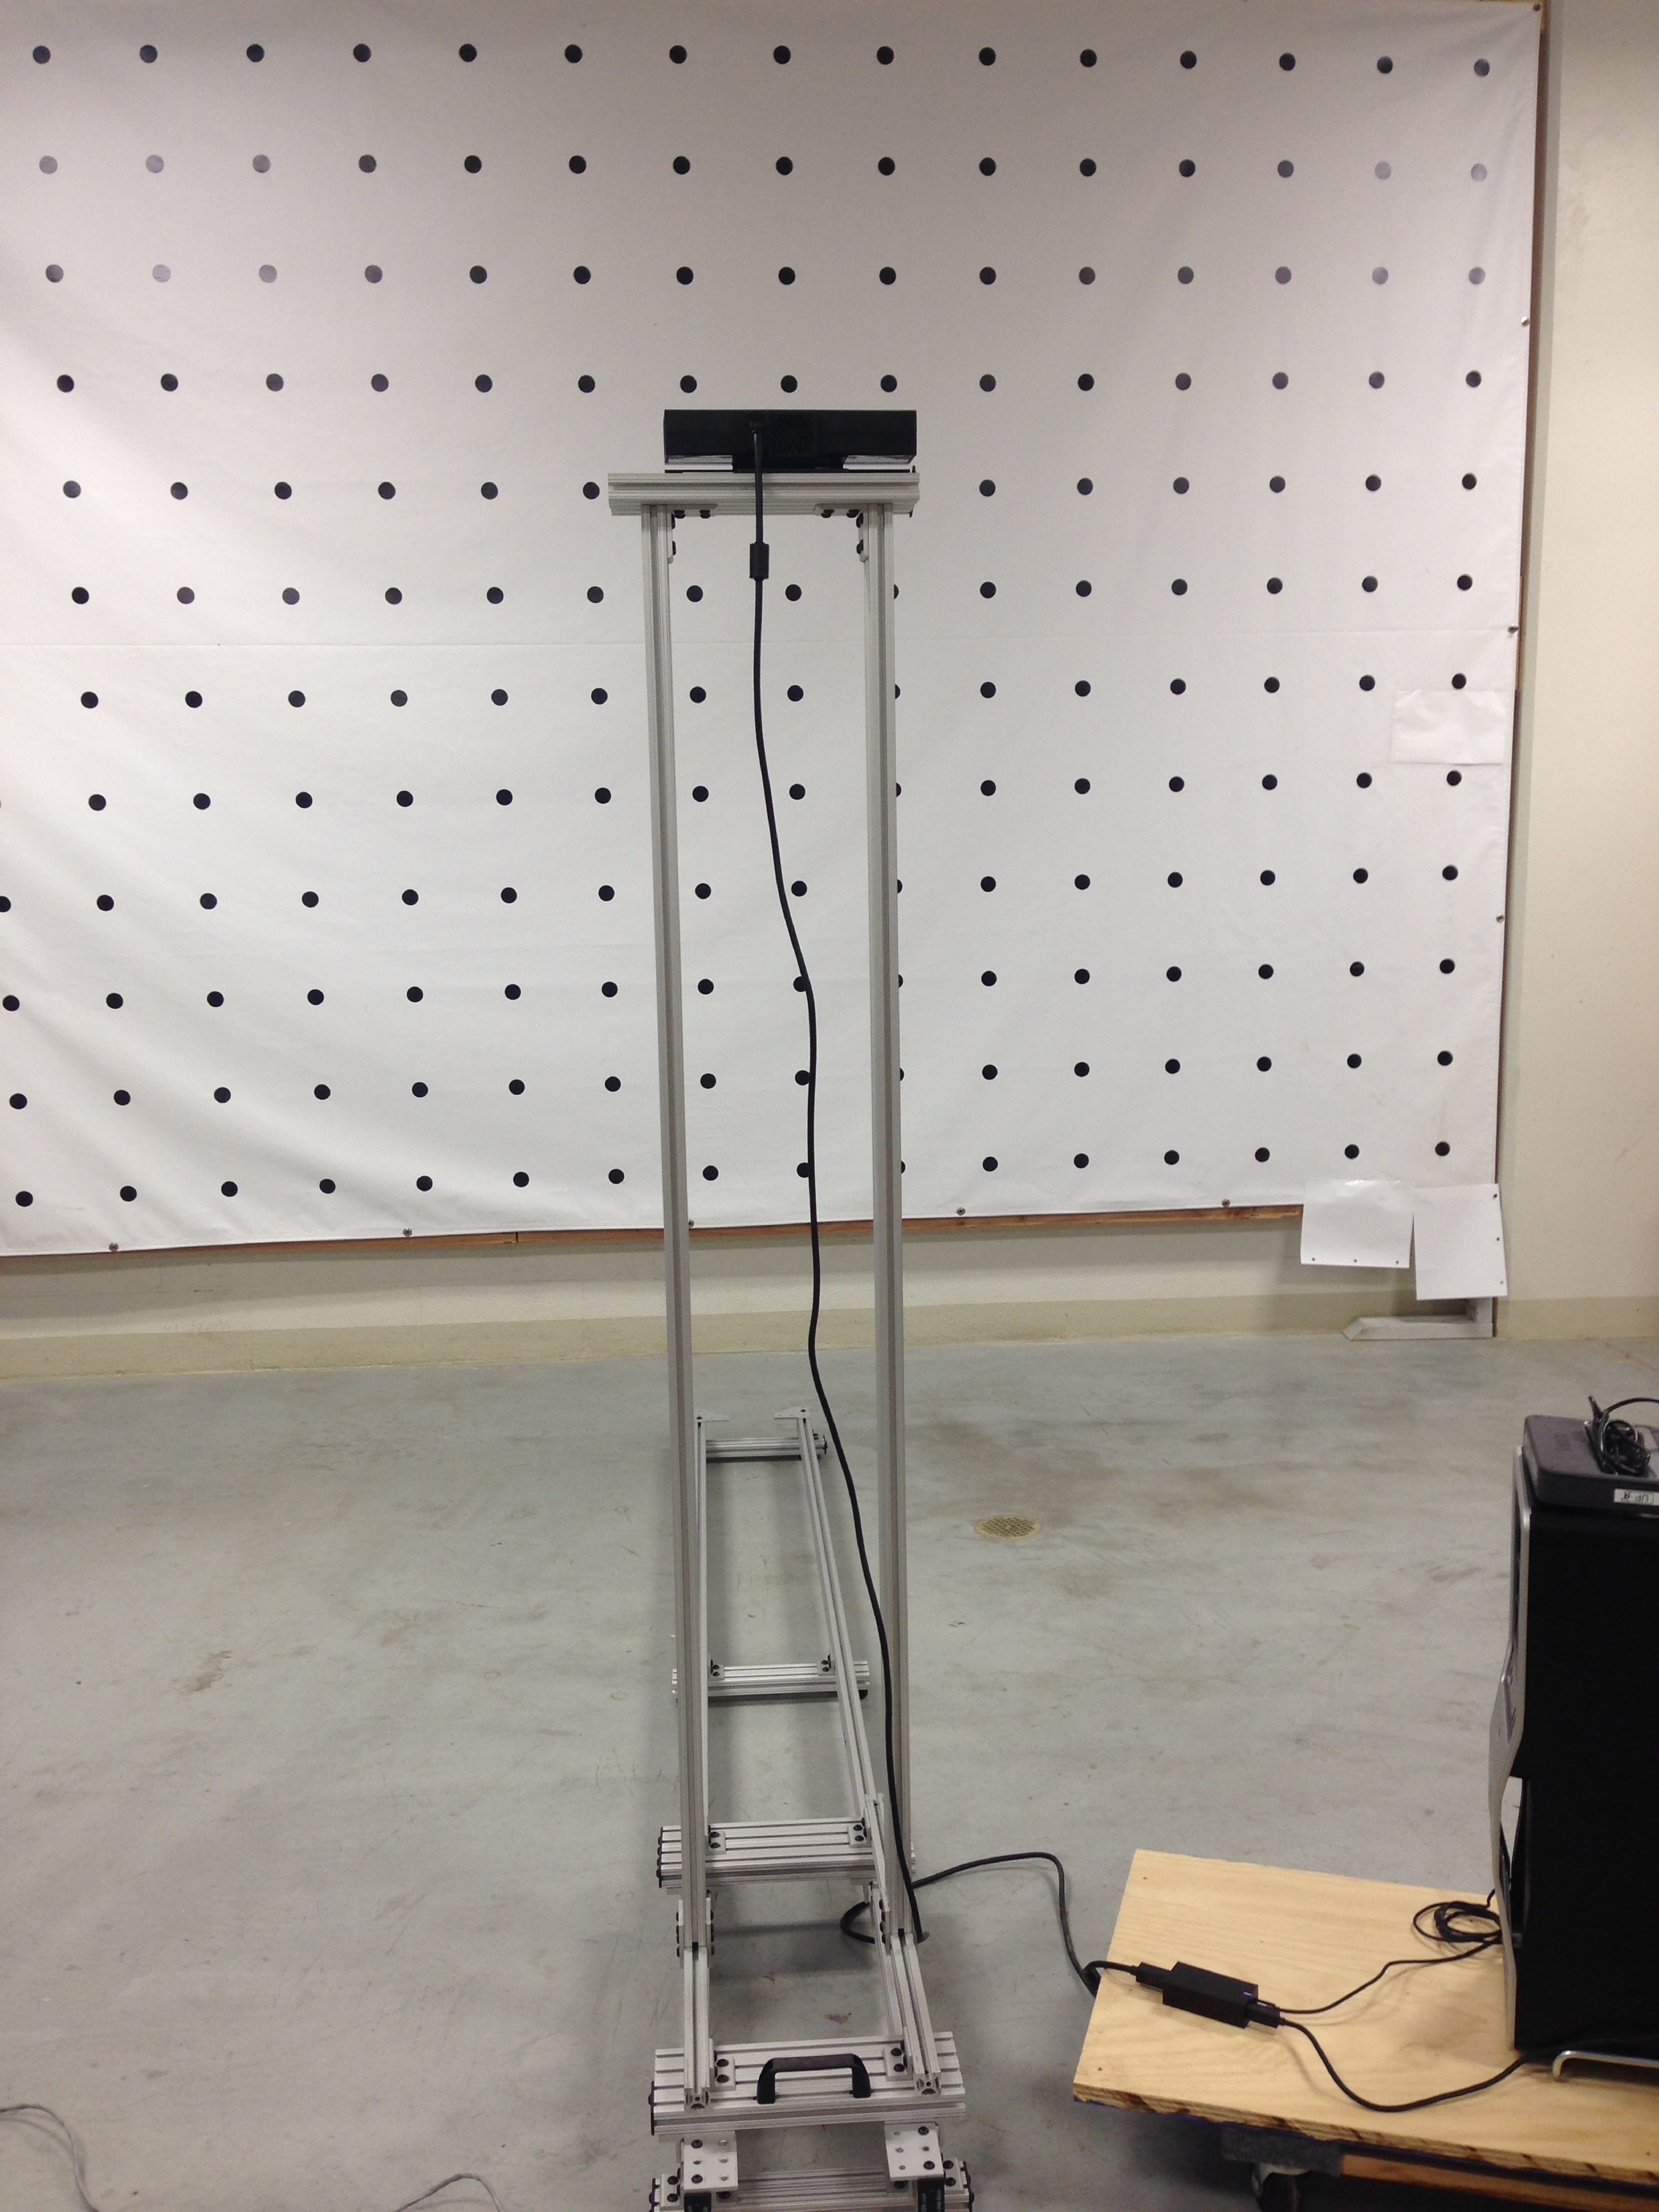
\includegraphics[width=0.55\textwidth]{trackingModuleOnKinectV2CalibrationSystem}
\caption{\gls{KinectV2} Calibration System}
\label{trackingModuleOnKinectV2CalibrationSystem}
\end{figure}%
Undistorted world space coordinates \(\gls{worldX}/\gls{worldY}/\gls{worldZ}\) with \(\gls{D}\) together will be collected and saved onto local drives, during which lens distortions will be removed. Instead of using the combination of pinhole-camera matrix and distortion removal vector, we will determine a best-fit, two--dimensional, high-order polynomial mapping that can directly map from \(Row\) (\(\gls{imageRow}\)) and \(Column\) (\(\gls{imageColumn}\)) in image space to \(\gls{worldX}\) and \(\gls{worldY}\), and the high-order polynomial mapping will handle the lens distortions. After the data collection, we will determine a best-fit mapping model between per-pixel \(\gls{D}\) and \(\gls{worldZ}\), and then process the collected data, and finally generate per-pixel mapping parameters, which can make up a look-up table that will help draw undistorted \gls{3D} reconstruction on \gls{GPU} in real-time.
\\\indent
In Chap.~\ref{chapterTraditionalCalibration}, a pinhole-camera-model based calibration method is discussed in detail, including the lens distortions analysis and its removal. Chapter~\ref{chapterDataBasedCalibration} will introduce how to draw the camera space \gls{3D} reconstruction on \gls{GPU}, introduce a rail calibration system's set-up, and then talk about the proposed per-pixel calibration method and simple \gls{3D} reconstruction on \gls{GPU} in detail. Chapter~\ref{chapterCaliResultsReconstruction} will explain how the two polynomial mapping models in the proposed calibration method are determined, and then show the calibrated results about how well the lens distortions and \emph{depth distortion} are corrected. Chapter~\ref{chapterConclusionAndFutureWork} will conclude this thesis and talk about the future work of \gls{RGBD} cameras calibration.


































































